\documentclass[global,twocolumn]{svjour}
%\documentclass[global,twocolumn,referee]{svjour}
% Remove option referee for final version
%
% Remove any % below to load the required packages
%\usepackage{latexsym}
\usepackage{graphics}
\usepackage{graphicx}
\usepackage{amssymb} 
\usepackage{amsmath}
% etc
%
% Insert the name of "your" journal with the command below:
\journalname{Applied Physics B}
%
\begin{document}
	%
\title{Silicon isotope separation in a SiF$_{4}$ molecular jet by two-frequency IR multiphoton dissociation}
	%\subtitle{Do you have a subtitle?\\ If so, write it here}
	\author{M Risaro\inst{1} \and V D'Accurso\inst{1} \and J Codnia\inst{1}% etc
		% \thanks is optional - remove next line if not needed
		\thanks{\emph{Present address:} Insert the address here if needed}%
	}                     % Do not remove
	%
	\offprints{}          % Insert a name or remove this line
	%
	\institute{DEILAP-CITEDEF-CONICET}
	%
	\date{Received: date / Revised version: date}
	% The correct dates will be entered by the editor
	%
	\maketitle
	%
\begin{abstract}
We performed Silicon isotope separation SiF$_{4}$ in a molecular jet by two frequency infrared multiphoton dissociation, using two TEA CO$_{2}$ laser. The dissociation process was monitored with a Time-of-Flight mass spectrometer by UV multiphoton ionization, using the fourth harmonic of a pulsed Nd:YAG laser. The dissociation yield and enrichment factor has been studied in terms of the lasers fluence, wavenumber and delay time. The results shows a remarkable increase in the dissociation yield and enrichment factor in the two-frequency technique compare with the single-frequency IRMDP.
\end{abstract}
	%
\section{Introduction}
\label{intro}

\textbf{Silicon isotope enrichment}

\textbf{Laser Isotope techniques}

\textbf{Infrared multiphoton ionization for silicon compounds}

\textbf{Two-frequency multiphoton ionization}

We have studied the two-frequency IRMPD of SiF$_{4}$ in a molecular jet. The dissociation eficiency and the enrichment factor were characterized with time of flight mass spectrommetry (TOF). The analysis of those main characteristics required the definition of estimators that disccount the background signal.  

\section{Experimental approach}
\label{sec:exerimental_approach}

A scheme of the experimental setup is shown in Figure \ref{fig:setup}. Two home-built TEA CO$_{2}$ laser were used as the excitation and dissociation sources. The excitation laser was tuned close to the Si-F stretching mode ($\nu_{3}$) to perform a vibrational excitation of the molecule. Furthermore, the dissociation laser was red shifted to a lower wave number from the $\nu_{3}$ vibrational mode. Both lasers have stable optical resonators and are focused through a 10 cm focal length ZnSe lens, in a collinear configuration.     

\begin{figure}[h]
	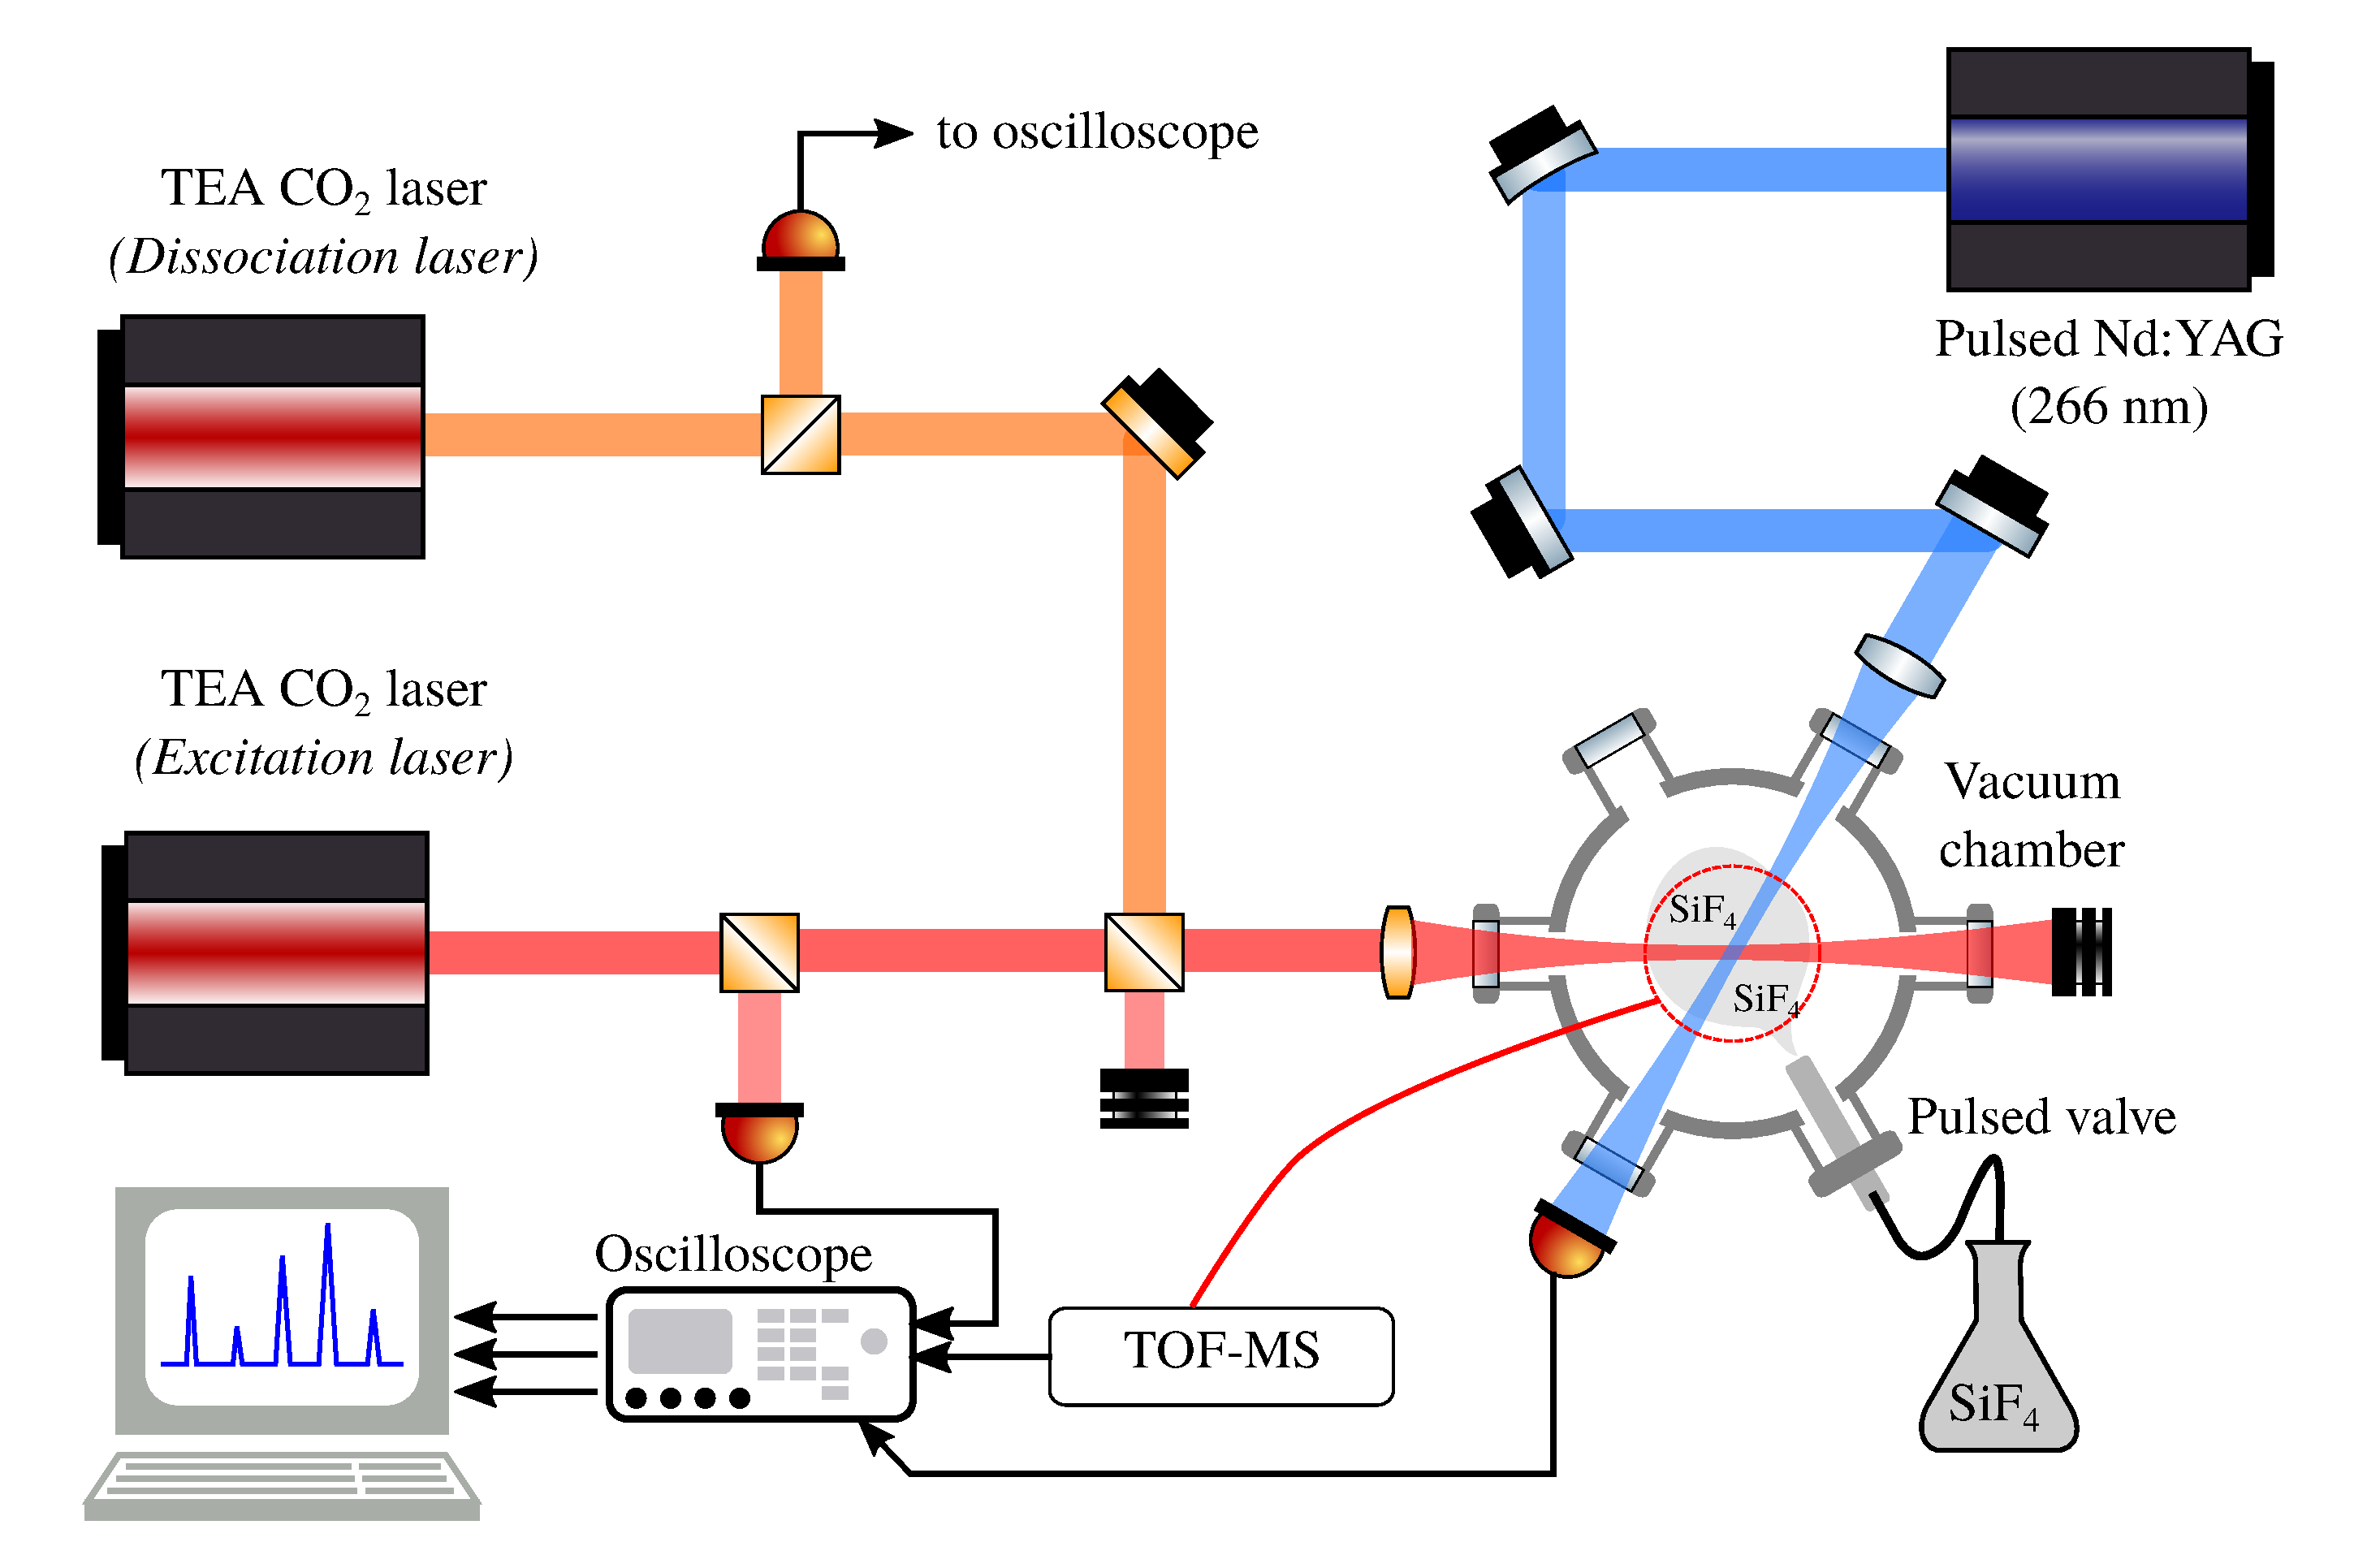
\includegraphics[width = 0.5\textwidth]{figures/dispositivo_2f_english.pdf}% Here is how to import EPS art
	\caption{\label{fig:setup} Experimental setup for the two frequency IRMPD over a molecular jet of SiF$_{4}$.}
\end{figure}

A sample of SiF$_{4}$ (99 \% Matheson) at a total pressure of 500 Torr was expanded through a pulsed valve (Parker Hannifin Corporation) into a stainless steel vacuum chamber, evacuated by a turbo-molecular pump (pump Brand). The average pressure in the molecular jet is estimated to be less than 1x10$^{-4}$ Torr \cite{bishop09}. Downstream, the molecular jet is crossed by the excitation and dissociation lasers and the ionization laser.

The generated ions are collected by an extractor potential into a Time of Flight Mass Spectrometer (Kore Technology) until they reach the ion detector. The obtained spectrum signals were recorded by an oscilloscope (Tektronix,DPO 7104 1GHz). We operate the CO$_{2}$ lasers at 1 Hz and the UV ionization laser at 2 Hz in order to discount the background on alternative shots. 

\subsection{Mass Spectrum analysis}

The irradiation of the molecular jet by the 266 nm UV laser produce a ionization but also a fragmentation of the SiF$_{4}$. Figure \ref{fig:spec_uv} shows a typical mass spectrum of the sample irradiated only by the UV laser. This pattern has no peak in the 104 mass, which implies that it has no parent. Also it can be seen that the highest peak corresponds to the [SiF$^{+}$] ion so the amplitude of the peak is used as an estimator of the concentration.     
\begin{equation}
\text{SiF$_{4}$} \xrightarrow{h \nu_{uv}}
\begin{cases}
\text{SiF$_{3}$$^{+}$} + \text{F} + e^{-} \\
\text{SiF$_{2}$$^{+}$} + \text{2F} + e^{-} \\
\text{SiF$_{1}$$^{+}$} + \text{3F} + e^{-} \\
\text{Si$^{+}$} + \text{4F} + e^{-}
\end{cases}
\end{equation}

\begin{figure}[h]
	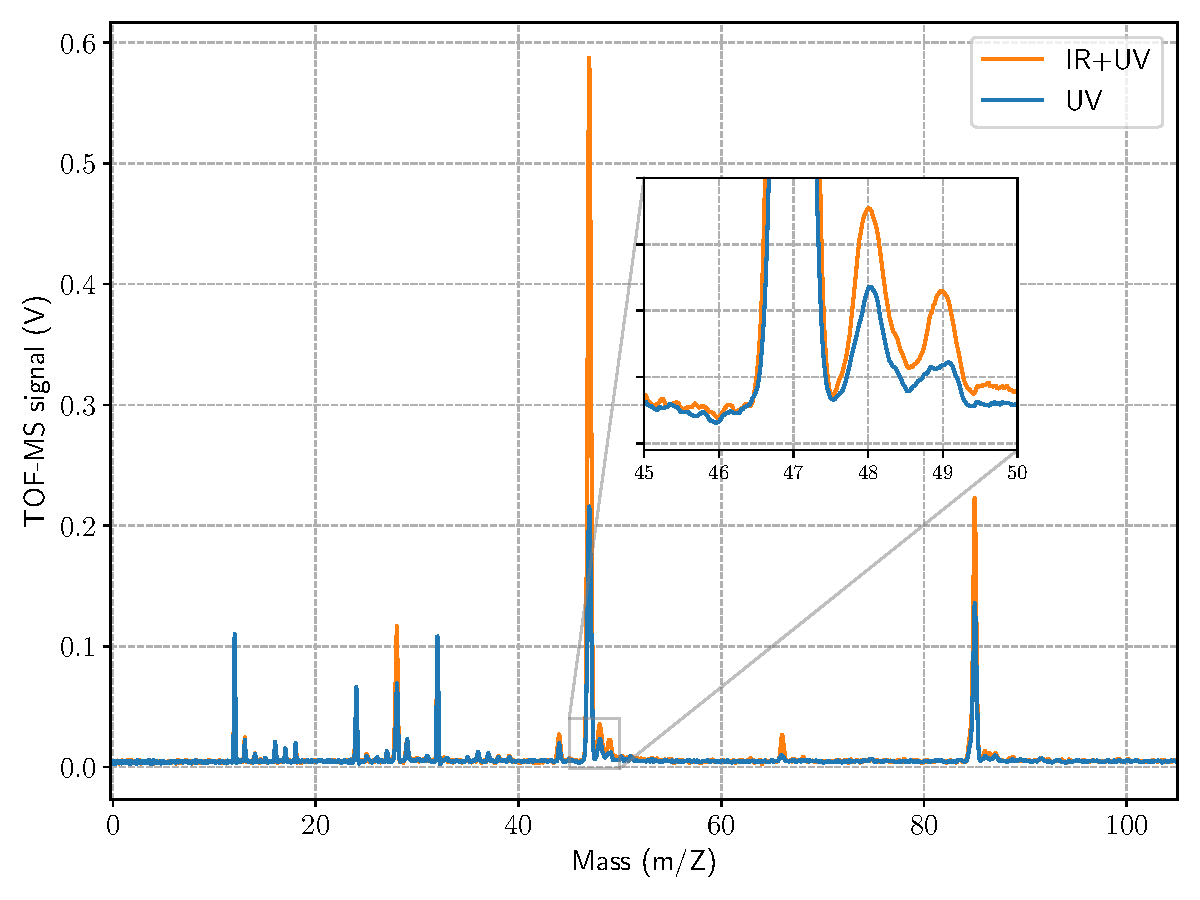
\includegraphics[width =1\linewidth]{figures/sp_uv_ir.pdf}
	\caption{\label{fig:spec_uv} SiF$_{4}$ mass spectrum obtained with 266 nm multi-photon ionization.}
\end{figure}

In the following experiments the SiF$_{4}$ molecular jet is first irradiated by IR radiation, to dissociate the molecule, and then the came the UV ionization to analyze the fragments in the TOF-MS. The IR lasers performs the following dissociation probability ($f^{i}$) for each isotope specie,

\begin{equation}
\text{SiF$_{4}$} \xrightarrow{\,\,\, h\nu_{\text{IR}} \,\,\,}
\begin{cases}
[^{28}\text{SiF$_{3}$}] = f^{28}[\text{SiF$_{4}$} ] \\
[^{29}\text{SiF$_{3}$}] = f^{29}[\text{SiF$_{4}$} ] \\
[^{30}\text{SiF$_{3}$}] = f^{30}[\text{SiF$_{4}$} ]
\end{cases}
\end{equation}
After this fragmentation, the sample is irradiated with the UV laser to ionize the sample but it also leads to another fragmentation. 
\begin{equation}
\text{$^{j}$SiF$_{4}$} \xrightarrow{h \nu_{IR}} \text{$^{j}$SiF$_{3}$+ F} \xrightarrow{h \nu_{UV}} \text{$^{j}$SiF$^{+}$+ 3F}  
\end{equation}

Summarizing, the total signal (I$^{T}$) in the SiF$^{+}$ is a combination of both processes. 
\begin{equation}
I^{T} = K \text{p}_{\text{SiF$_{3}$}}^{\text{SiF$^{+}$}} f^{28}[\text{SiF$_{4}$}] + \text{K} \text{p}_{\text{SiF$_{4}$}}^{\text{SiF$^{+}$}} (1-f^{28})[\text{SiF$_{4}$}]
\end{equation}
where K is an instrument constant, related to the ion counting convertor and the data acquisition.

In order to characterize the dissociation yield of the IRMPD process, we define the $\alpha_{j}$ estimator. This is the ratio between the total mass spectrum and the UV spectrum.
\begin{equation}
\alpha_{j} = 
\begin{cases}
\alpha_{47} = (q-1)f^{28} \\
\alpha_{48} = (q-1)f^{29} \\
\alpha_{49} = (q-1)f^{30}
\end{cases}
\end{equation}

As can be seen, $\alpha_{j}$ is proportional to $f^{j}$ and q is the ratio between ionization probabilities of SiF$_{4}$ and SiF$_{3}$. In the same way, is possible to define the isotope selectivity estimator $\beta$,
\begin{equation}
\beta_{k} = 
\begin{cases}
\beta_{29} = \frac{\alpha_{47}}{\alpha_{48}} = \frac{f^{28}}{f^{29}} \\
\beta_{30} = \frac{\alpha_{47}}{\alpha_{49}} = \frac{f^{28}}{f^{30}}
\end{cases}
\end{equation}


\textbf{Justificaci\'on para decir que vamos a analizar solamente el estimador $\alpha_{47}$ y el estimador $\beta_{30}$}
 
\section{Results and discussion}
\subsection{Delay time laser dependence}
The first parameter we analyzed in the IRMPD process was the delay between the TEA CO$_{2}$ lasers. The excitation laser is tuned to $\nu_{e}= 1031.5$ cm$^{−1}$ and the dissociation laser to $\nu_{D}=983$ cm$^{-1}$. The fluence for both lasers where $\Phi_{E}=120 $J/cm$^{2}$ and $\Phi_{D}=$ 120 J/cm$^{2}$. 

\begin{figure}[h]
	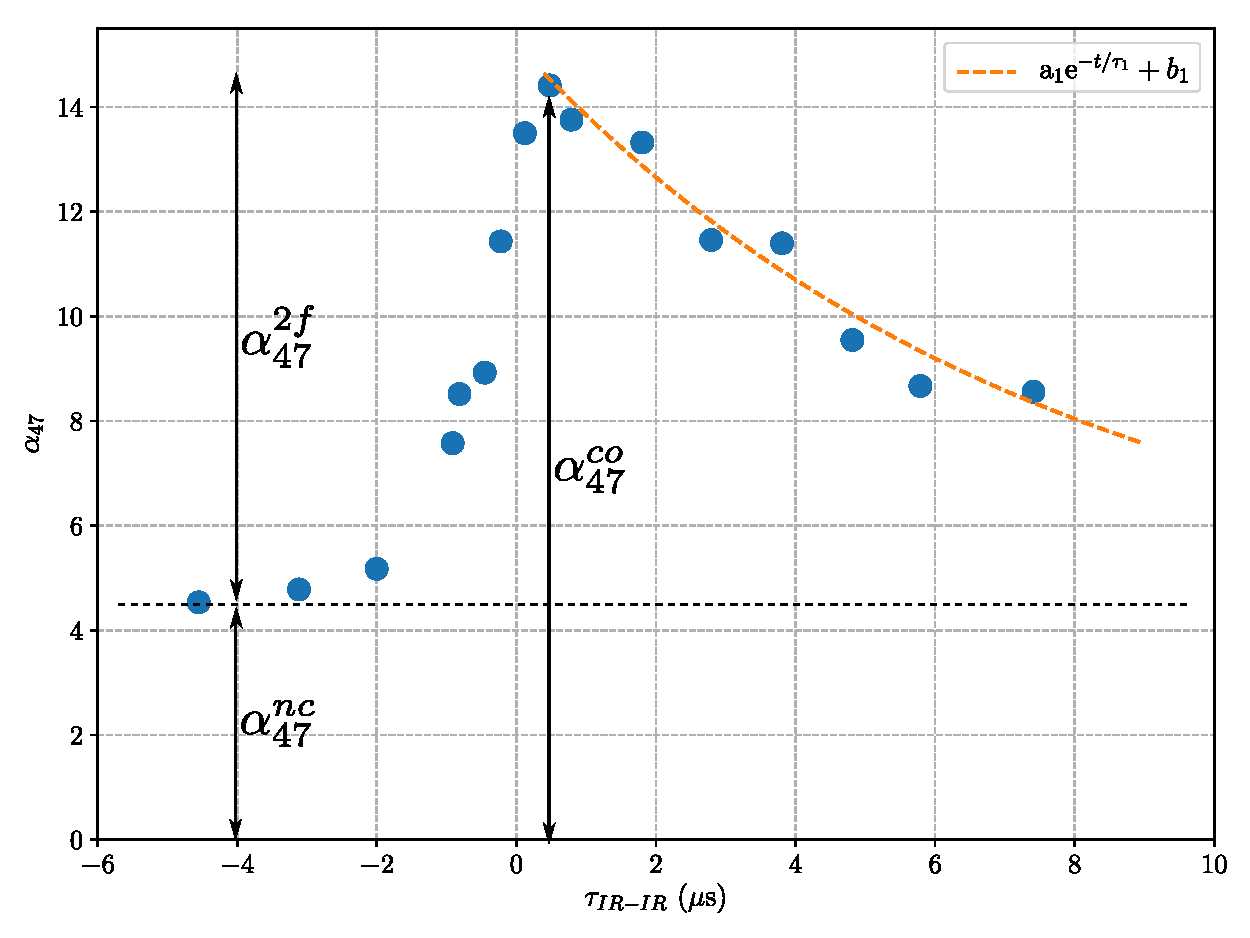
\includegraphics[width=1\linewidth]{figures/alfa_47_decaimiento.pdf}
	\caption{Pulse delay dependence of the dissociation yield ($\alpha_{47}$ estimator) We define de pulse delay relative to the begining of the excitation laser.}
	\label{fig:alpha_47_estimator}
\end{figure}

The $\alpha$ estimator shows a plateau for delay times between -4 $\mu$s and -2 $\mu$s, related to the dissociation rates of each IR laser. Since the overlap of the two pulses we find a peak in $\alpha$, due to the two-frequency IRMPD. As we mention in the previous section, the first IR laser send molecules to the quasi-continuum and the second dissociates those excited molecules.

In order to obtain the pure contribution of the two frequency process, we make alternative measurements of "cooperative" and "non cooperative" situations. In the first one both lasers overlaps in the time domain and the delay is close to zero. While in the non cooperative case the delay is around -4 $\mu$s. By making the difference of those situation we obtain $\alpha^{2f}$. 

\begin{equation}
\begin{split}
\alpha^{co} &\leadsto \alpha^{2f} + \alpha^{E} + \alpha^{D} \\
\alpha^{nc} &\leadsto \alpha^{E} + \alpha^{D}
\end{split}
\label{alfa_47_co}
\end{equation}  

Figure \ref{fig:alpha_47_estimator} also shows the $\alpha$ decay which is fitted by an exponential function. The decay constant is $(7.8\pm0.4)$ $\mu$s, five times larger than the tail of the IR lasers pulse. However, this decay time is in full agreement with the transit time of the molecular jet through the irradiation volume[cita].  

\subsection{Laser fluence dependence}
In Figure \ref{fig:alpha_phi_excitation} we show the $\alpha^{2f}_{47}$ estimator's dependency with the dissociation laser fluence ($\Phi_{D}$). The experimental data is fitted by a power law function which is shown in orange dashed line. The exponent obtained is $a = 0.49\pm 0.02$, in full agreement with previous works [CITA GRUPO].  

\begin{figure}[h]
	\centering
	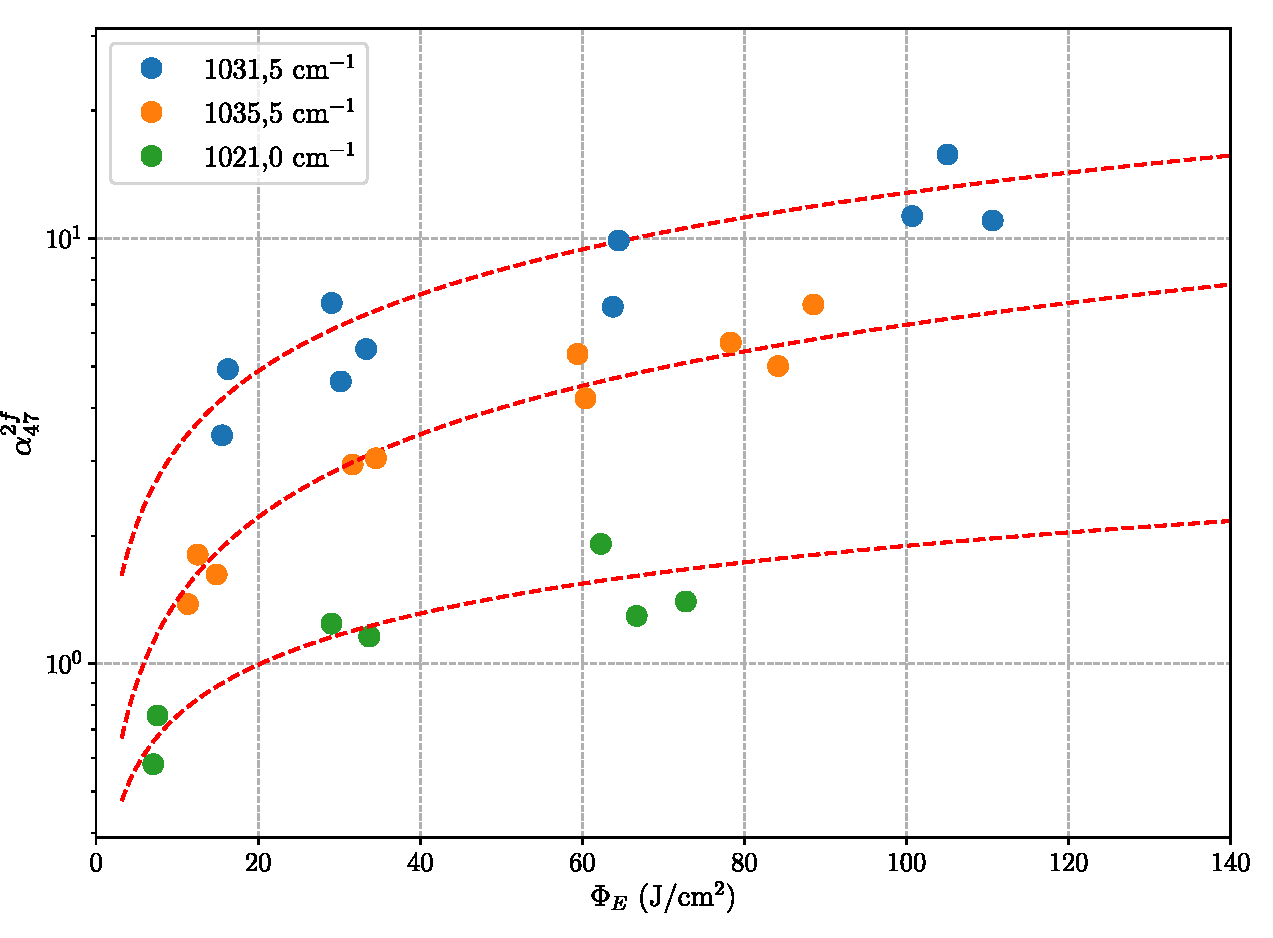
\includegraphics[width = 1\linewidth]{figures/alpha_47_phi_bombeo.pdf}
	\caption{ Dissociation yield estimator as a function of the dissociation laser fluence.}
	\label{fig:alpha_phi_excitation}
\end{figure}

Although the power law function fits the experimental data points, we are not able to reach a saturation of the dissociation estimator.  

\subsection{Laser wavenumber dependence}
In general, the IRMPD dissociation probability shows a red shifted compare with normal modes oscillation frequencies; mainly due to the vibrational anharmonicity. 

\begin{figure}[h]
	\centering
	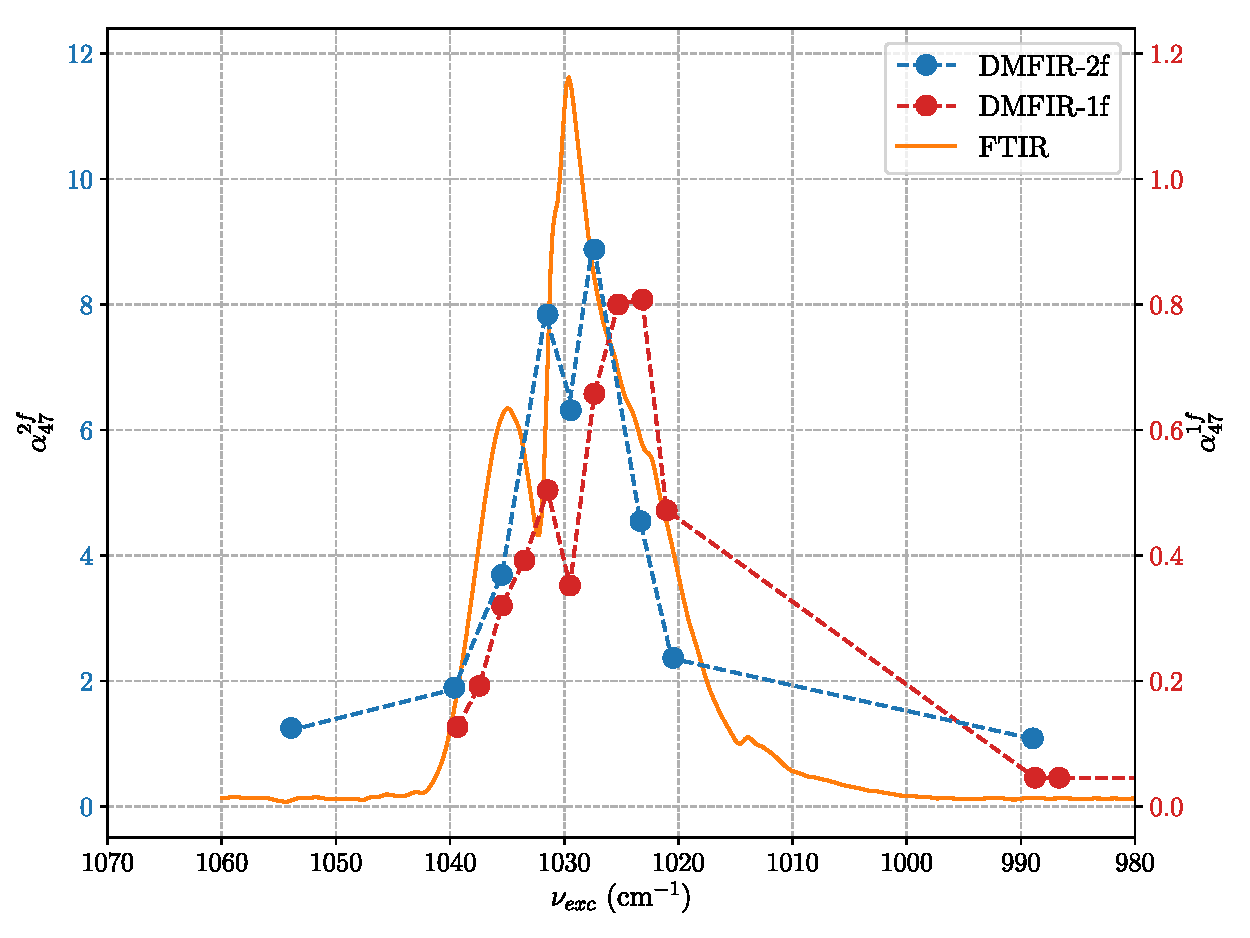
\includegraphics[width = 1\linewidth]{figures/alfa_47_nu_bombeo.pdf}
	\caption{\label{fig:alfa_nu_bombeo} Dependence of the $\alpha_{47}$ estimator on the excitation laser frequency (blue dots) compare with the linear absorption IR spectrum of SiF$_{4}$.}
\end{figure}

Figure \ref{fig:alfa_nu_diso} shows the $\alpha_{47}^{2f}$ estimator as a function of the dissociation laser wavenumber superimposed with the IR linear absorption spectrum. The fluences of the excitation and dissociation lasers were 50 J/cm$^{2}$ and 60 J/cm$^{2}$, and the delay was fixed at 1$\mu s$. As can be seen, the dissociation yield presents a resonance close to 980 cm$^{-1}$ which is almost 50 cm$^{-1}$ red-shifted compared to the IR linear absoprtion spectrum. This result indicates that the SiF$_{4}$ has been excited to the vibrational quasicontinuum by the excitation laser.  

As a rule of thumb we can assume a linear anharmonicity of the vibrational levels, founded on the Morse potencial. In the SiF$_{4}$ case, the anharmonicity constant is $\chi_{e}\nu_{3} \simeq 5 \text{cm}^{-1}$, so we can estimate that the molecule has been excited up to the $\nu_{SF} = 10$. 

\begin{figure}[h]
	\centering
	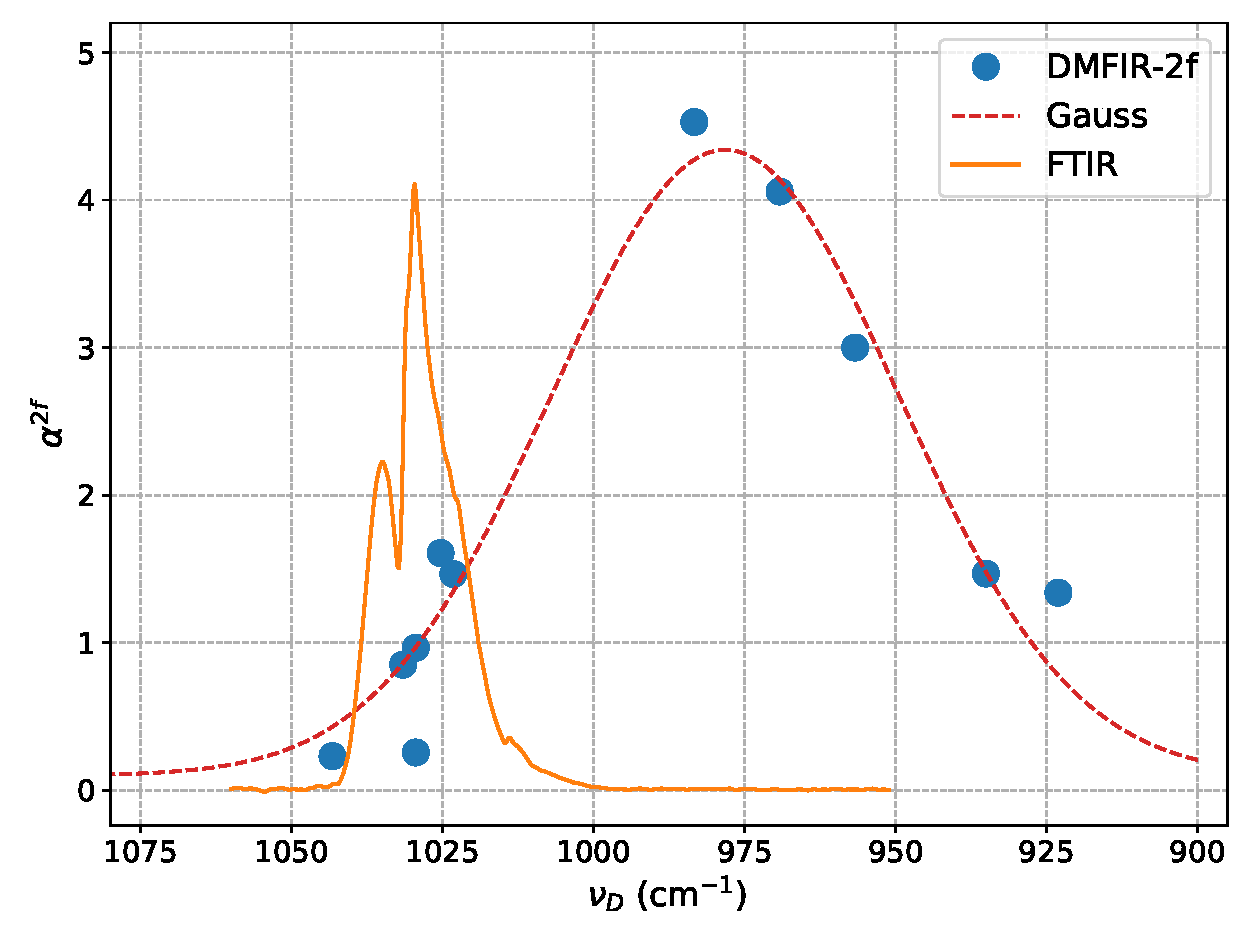
\includegraphics[width = 1\linewidth]{figures/alfa_47_nu_diso.pdf}
	\caption{\label{fig:alfa_nu_diso} Dependence of the $\alpha_{47}$ estimator on the dissociation laser frequency (blue dots) together with a gaussian distribution fit (orange dashed line), and the linear absorption IR spectrum of the $\nu_{3}$ absorption line.}
\end{figure}

\subsection{Enrichment factor}
In Figure \ref{fig:beta_spec} the enrichment factor $\beta_{30}$ is plotted against the excitation and the dissociation wavenumber. The factor shows a resonance as a function of $\nu_{e}$ with an slightly red shift compared with Si-F stretching normal mode. On the other side, the resonance is shifted almost 50 cm$^{-1}$ in terms of the dissociation laser wavenumber. 

\begin{figure}[h]
	\centering
	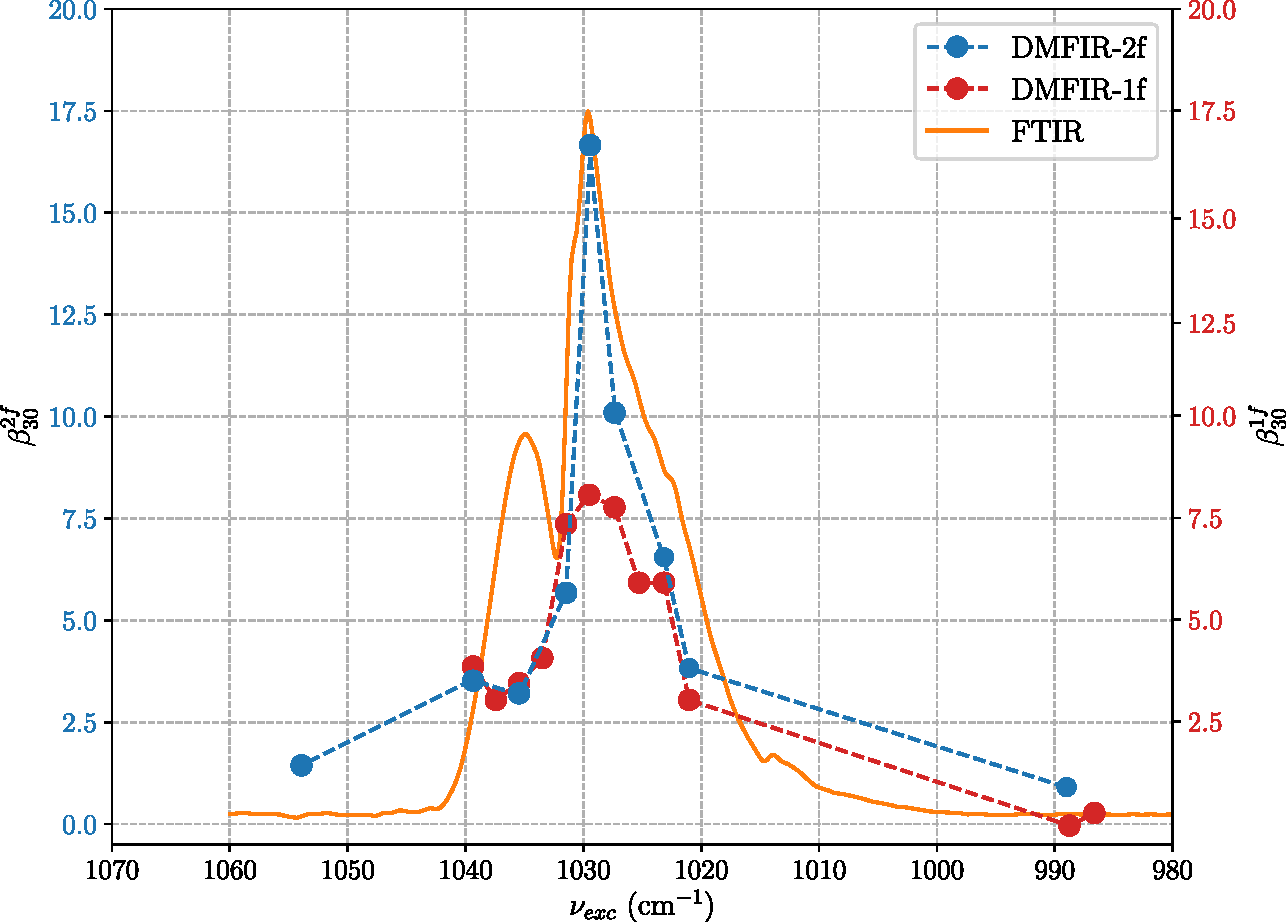
\includegraphics[width = 1\linewidth]{figures/beta_30_nu_bombeo.pdf}
	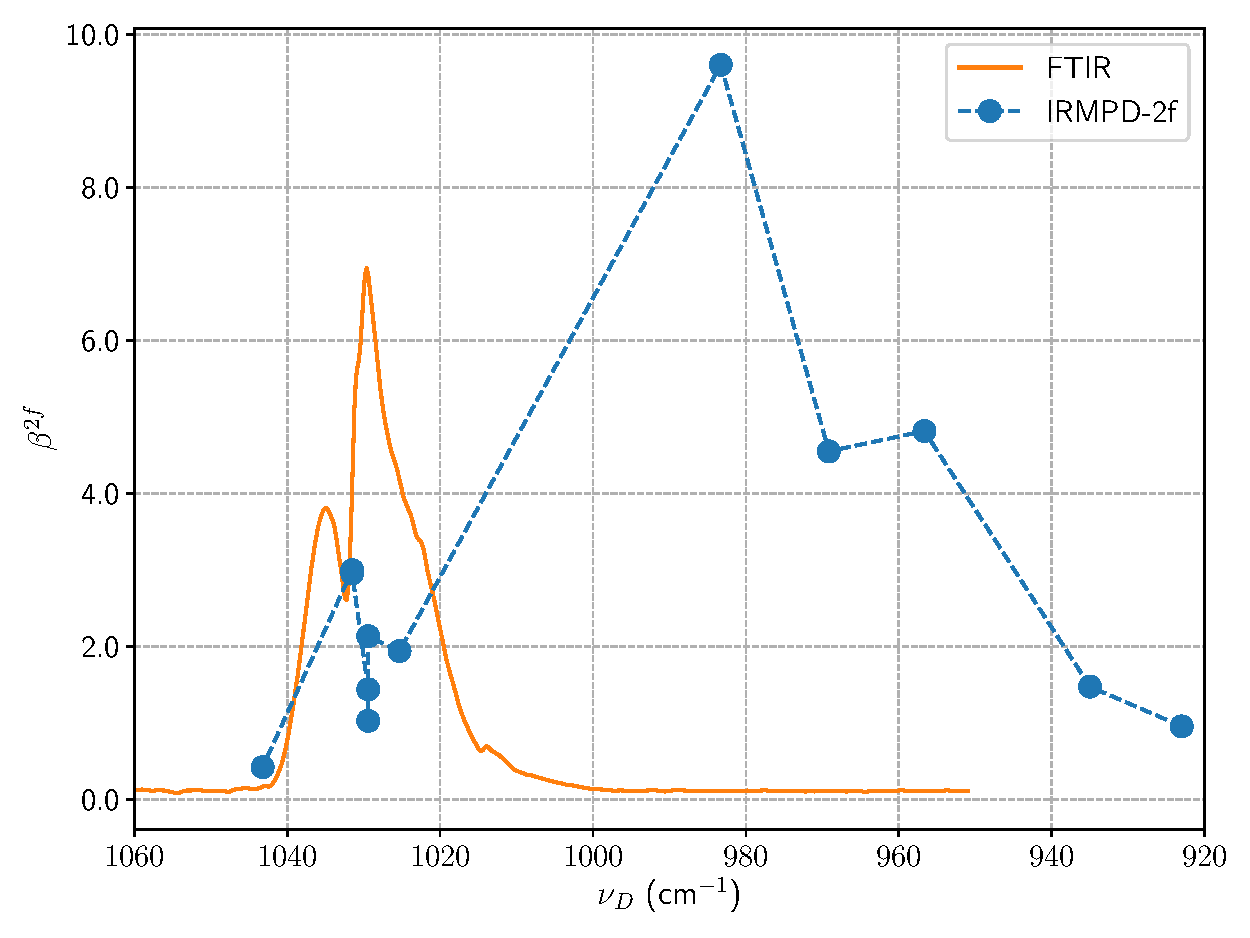
\includegraphics[width = 1\linewidth]{figures/beta_30_nu_diso.pdf}
	\caption{\label{fig:beta_spec} Isotope enrichment factor as a function of lasers wavenumber. In the upper plot we show $\beta_{30}$ dependence with the excitation laser wavelenegth. Below, the $\beta_{30}$ as a function of the dissociation laser wavelength. Both are compared with the IR linear absorption spectrum of SiF$_{4}$.}
\end{figure}

\textbf{Comment about the improvement of the $\beta$ estimator}

\section{Conclusions}
	% BibTeX users please use
	% \bibliographystyle{}
	% \bibliography{}
	%
	% Non-BibTeX users please use

\begin{thebibliography}{}
	%
	% and use \bibitem to create references.
	%
	\bibitem{RefJ}
	% Format for Journal Reference
	Author, Journal \textbf{Volume,} (year) page numbers.
	% Format for books
	\bibitem{RefB}
	Author, \textit{Book title} (Publisher, place year) page numbers
	% etc
\end{thebibliography}
	
	
\end{document}

% end of file template.tex
